\documentclass[a4paper,12pt]{jsarticle}

\usepackage{amsmath,amssymb}
\usepackage{bm}
\usepackage[dvipdfmx]{graphicx}
\usepackage{verbatim}
\usepackage{wrapfig}
\usepackage{ascmac}
\usepackage{makeidx}
\usepackage{multirow}
\usepackage{here}
\usepackage{url}
\usepackage{comment}
%\usepackage{color}
\usepackage{arydshln}
\usepackage[top=35truemm,bottom=35truemm,left=25truemm,right=25truemm]{geometry}

%\renewcommand{\figurename}{Fig.}

\title{システム創造プロジェクト 最終レポート}
\author{第5班}
\date{\today}

\begin{document}

\maketitle

\section{基本情報}
\subsection{プロジェクト名}
{\large 動画変換システム\ 〜骨格推定等を用いた新時代の政治エンタメの提案〜}

\subsection{メンバー}
\begin{table}[H]
    \begin{tabular}{cl}
        19M11893 & 岩本 拓也\\
        19M12220 & 藤本 八雲\\
        19M18323 & 倉林 快生\\
        19M12065 & 田屋 裕輝\\
        19M12160 & 林 良優\\
        19M11982 & 岸 良樹\\
        19M12295 & 森本 義弥
	\end{tabular}
\end{table}

\subsection{概要}

現代の日本が抱える問題の一つに, 選挙における若者の投票率の低さが挙げられる.
本プロジェクトでは, 政治への関心を高めることを目的として, 骨格推定等を用いて政見放送等の動画をVTuberの動画に変換するシステムを作成した.

\begin{figure}[H]
	\begin{center}
		\begin{tabular}{c}
			\begin{minipage}{0.50\hsize}
				\centering
				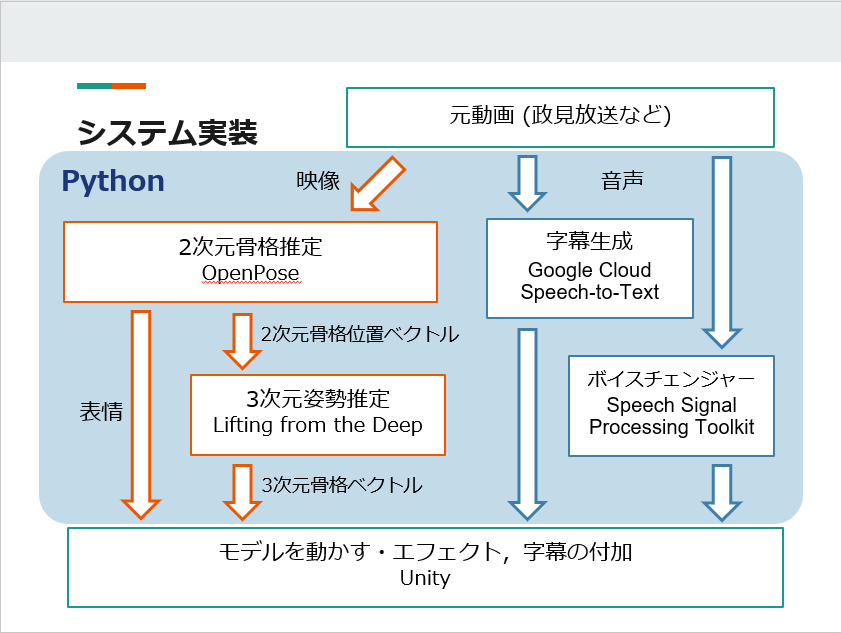
\includegraphics[width=7.5cm]{./fig/slide1.png}
				% \caption{}
				% \label{}
			\end{minipage}

			\begin{minipage}{0.50\hsize}
				\centering
				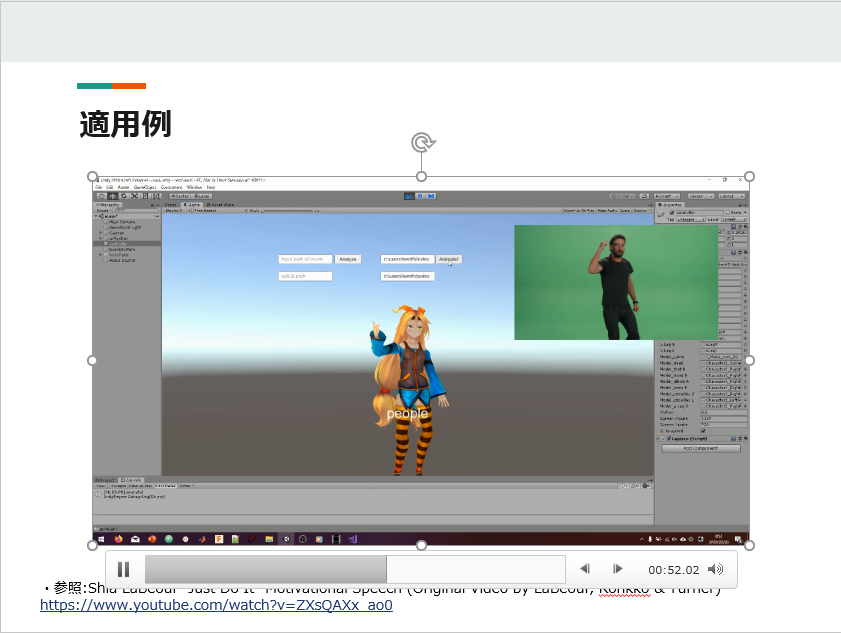
\includegraphics[width=7.5cm]{./fig/slide2.png}
				% \caption{}
				% \label{}
			\end{minipage}
		\end{tabular}
		% \label{}
	\end{center}
\end{figure}

\section{製作したソフトウェア}
\subsection{ソフトウェアの使用方法}
\subsubsection{環境のセットアップ}
本製品の使用には以下のハードウェア環境が必要となる.
\begin{itemize}
  \item Windows10(64-bit) machine
  \item CUDA対応GPU
\end{itemize}

加えて以下のソフトウェア環境が必要となる.
\begin{itemize}
  \item Python3.X (Anaconda3の最新バージョンに対応したものを推奨)
  \item Anaconda3
  \item Unity editor
  \item CUDA toolkit v9.0
  \item CUDNN 7.0.5
  \item Openpose v1.4.0
  \item Lifting from the Deep
\end{itemize}

同梱のバッチファイルを利用することで環境構成負担は大幅に軽減されている.紙面の都合上,実行環境のセットアップに関しての詳細は\url{https://github.com/syspro5/iwamoto}を参照のこと.


\subsubsection{実行方法}
\begin{enumerate}
  \item unityエディタを起動し,本製品のプロジェクトファイルを開く.
  \item 解析したい動画のパスを指定する.
  % \begin{figure}[h]
  %   \centering
  %   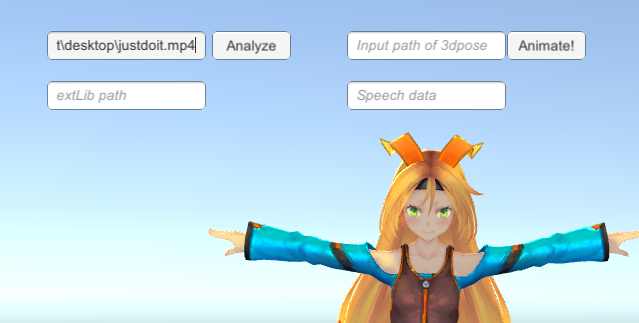
\includegraphics[width=1.0\textwidth]{fig/iw1131.png}
  %   \label{fig:iw1131}
  % \end{figure}
  %\clearpage
  \item Analyzeボタンを押すと解析が開始され,結果ファイルが出力される
  % \begin{figure}[h]
  %   \centering
  %   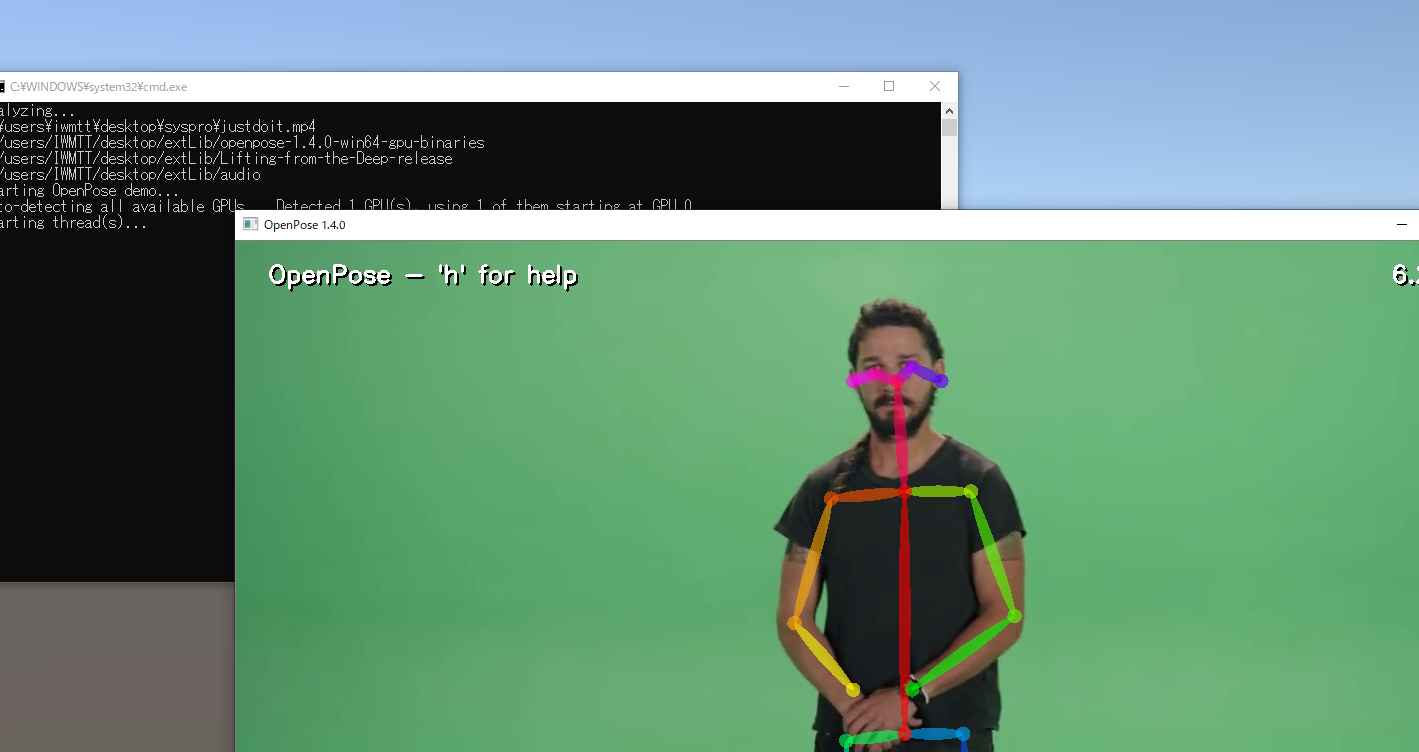
\includegraphics[width=1.0\textwidth]{fig/iw1132.png}
  %   \label{fig:iw1132}
  % \end{figure}
  \item 解析終了後Animateボタンを押すことで字幕とモデルの動きの動画が出力される.
%   \begin{figure}[h]
%     \centering
%     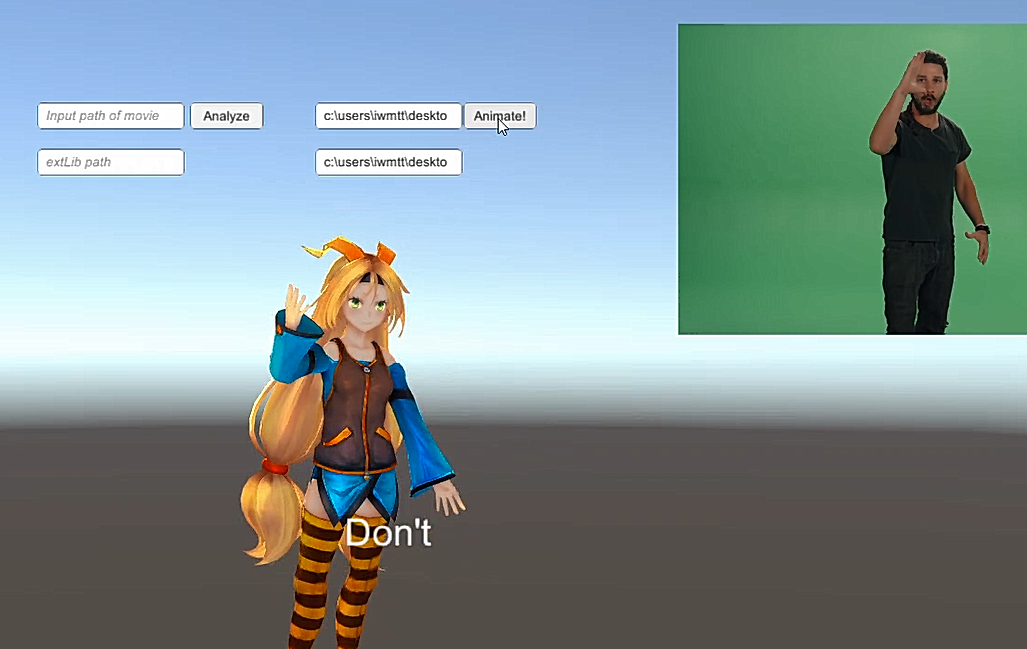
\includegraphics[width=1.0\textwidth]{fig/iw1133.png}
%     \label{fig:iw1133}
%   \end{figure}
\end{enumerate}
実際の実行の様子は同梱されたビデオファイルを参照のこと.

\begin{figure}[h]
    \centering
    \begin{tabular}{c}
      \begin{minipage}{0.3\hsize}
        \centering
        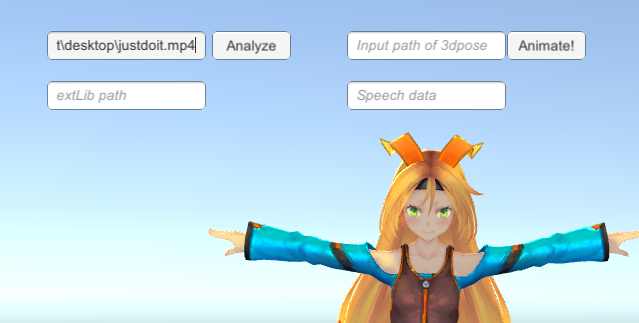
\includegraphics[width=1.0\textwidth]{fig/iw1131.png}
        \text{解析したい動画のパス指定}
      \end{minipage}

      \begin{minipage}{0.3\hsize}
        \centering
        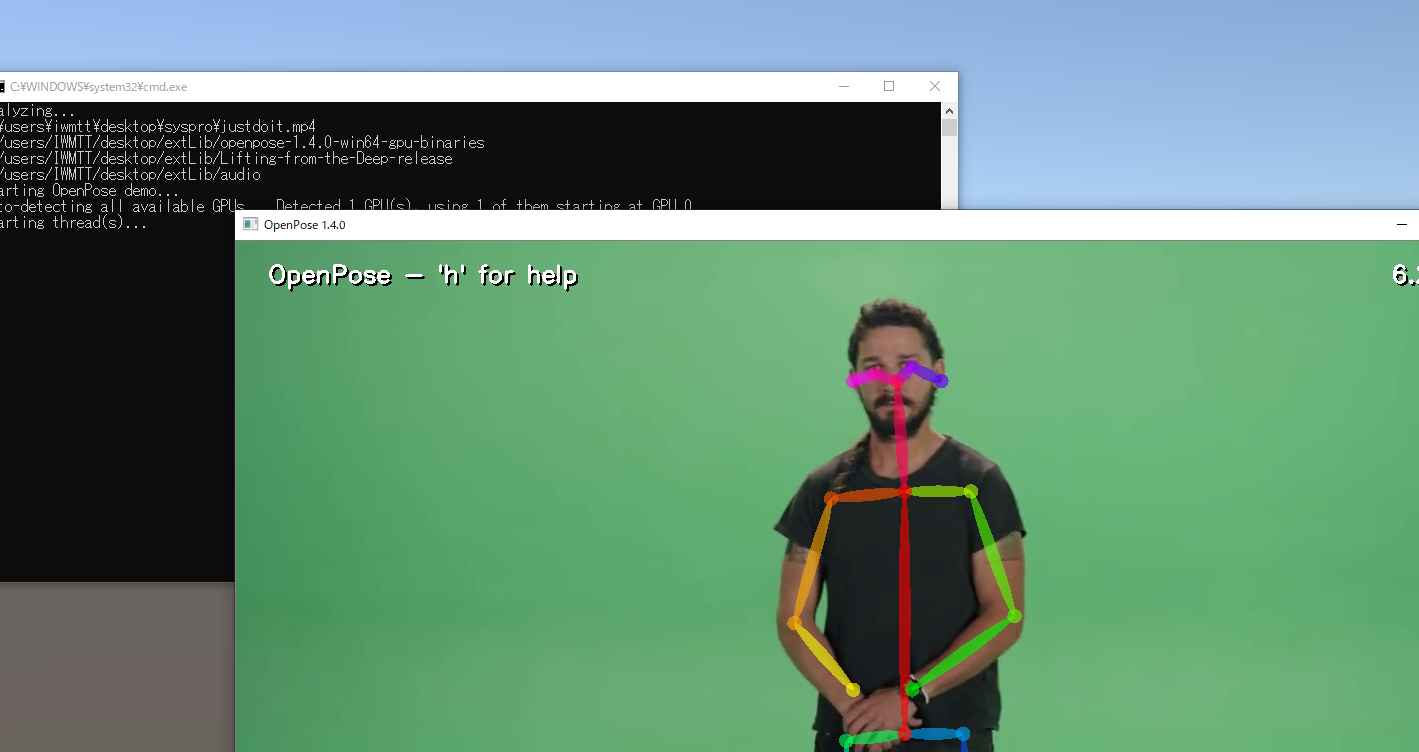
\includegraphics[width=1.0\textwidth]{fig/iw1132.png}
        \text{処理中の画面}
      \end{minipage}

      \begin{minipage}{0.3\hsize}
        \centering
        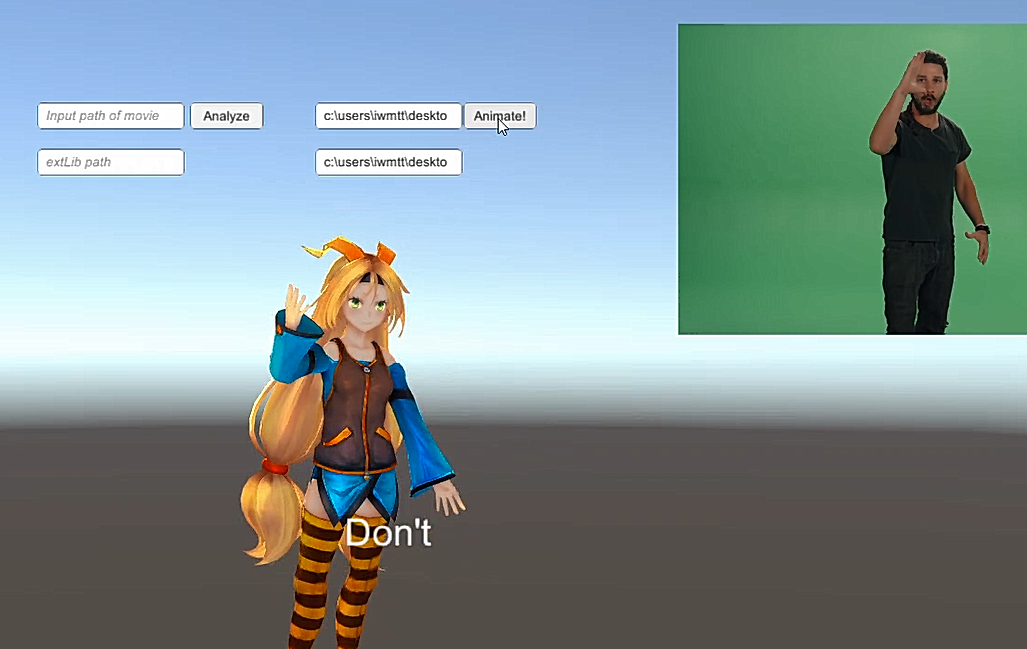
\includegraphics[width=1.0\textwidth]{fig/iw1133.png}
        \text{実行結果}
      \end{minipage}

    \end{tabular}
    \caption{ミーティング内容の比較}
    \label{fig:iw113compare}
\end{figure}

\subsection{ソフトウェアの機能・仕様}
\begin{itemize}
  \item 深度情報なしに骨格推定を行い,モデルに動きを反映させる一連の処理を画一化.
  \item 音声解析により字幕描画も実装.
  \item 推定可能人数は実装時点では1人
  \item 現時点ではUnity editor上での実行となる

\end{itemize}

\subsection{ソフトウェアの設計・製作過程}
\subsubsection{設計}
処理のフローチャートを以下の図\ref{fig:iw1311}に示す.
動画から音声などを抽出し,要素ごとに分けて処理を行っている.
通常Unityから直接pythonの仮想環境へのアクセスはできないため,今回の実装ではシェルスクリプトを介してanacondaの仮想環境にアクセスする手法をとっている.
仮想環境をセットアップするスクリプトも同梱しているため,利用者が一々必要なライブラリをインストールする必要はない.
また,専用の仮想環境を作成することで,利用者のpython環境を改変することなしに複数のライブラリの利用が可能となることも利点となる.
\begin{figure}[h]
  \centering
  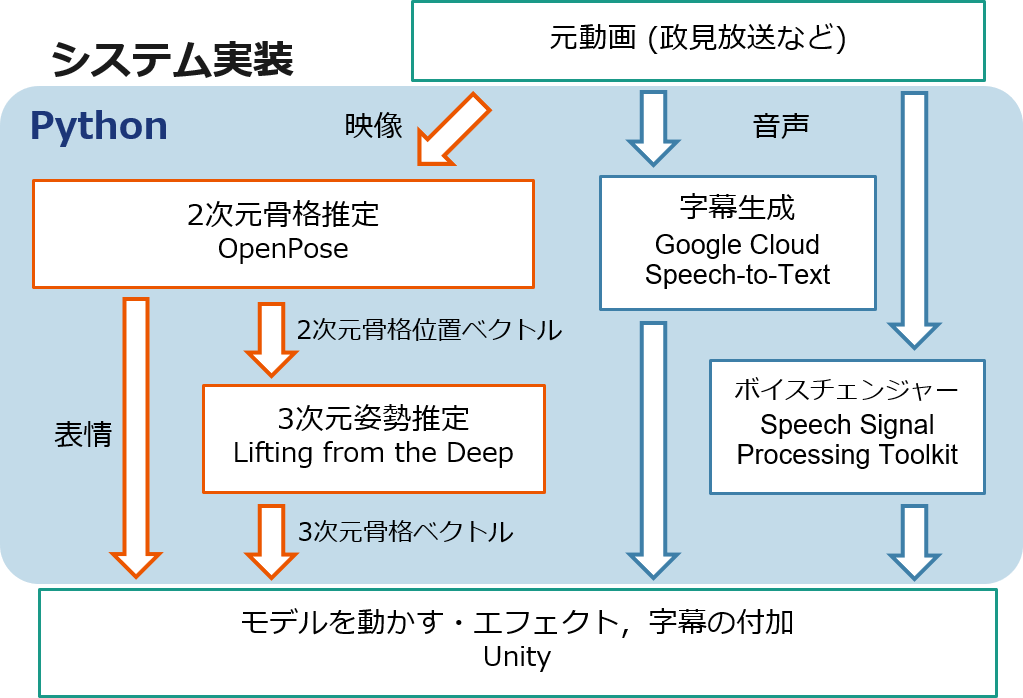
\includegraphics[width=1.0\textwidth]{fig/iw1311.png}
  \caption{処理の概要図}
  \label{fig:iw1311}
\end{figure}

\subsubsection{製作過程}
10月時点と12月時点でのミーティング事項の比較を図\ref{fig:iw132compare}に示す.
10月時点では定まっていなかった「具体的に何を使用するか」が,12月時点では明確に定まった.

\begin{figure}[h]
  \centering
 \begin{minipage}[b]{0.45\linewidth}
  \centering
  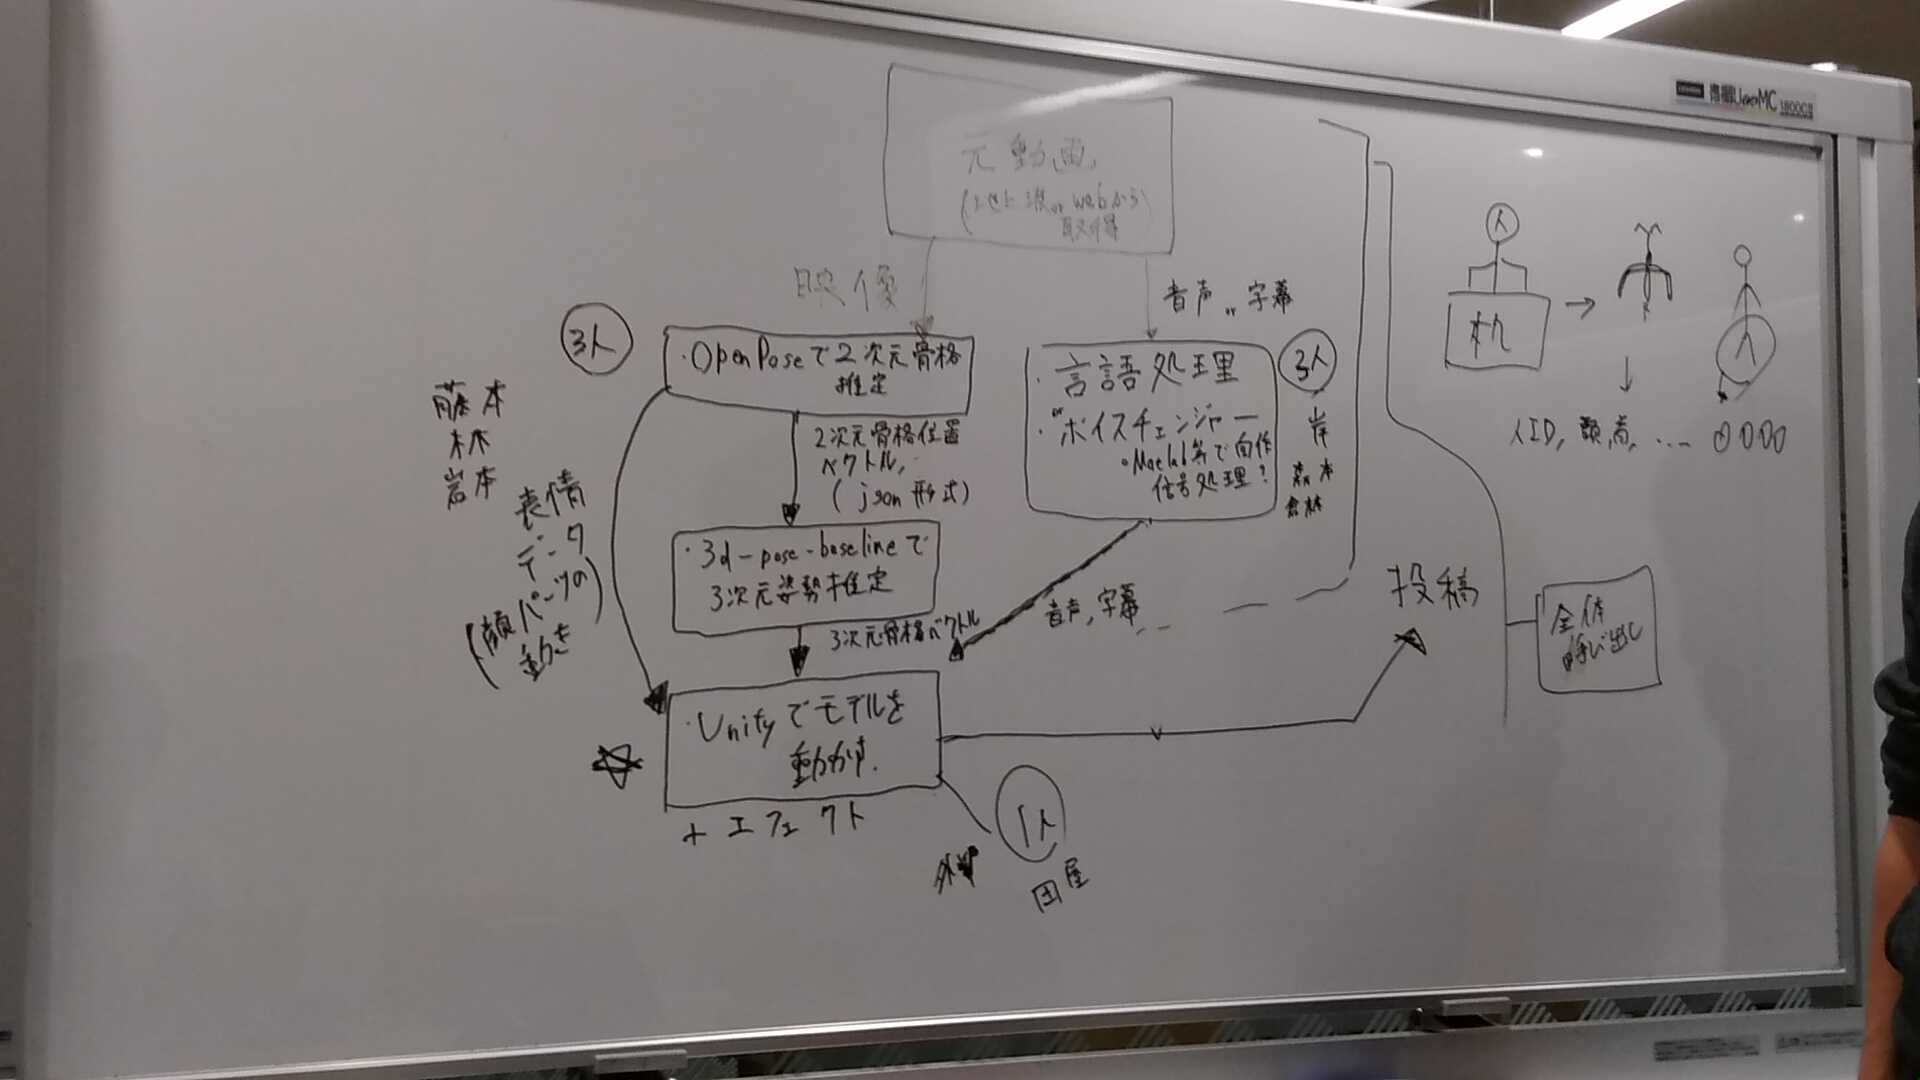
\includegraphics[width=1.0\textwidth]{fig/iw1321.png}
  \text{10月時点}
  \end{minipage}
 \begin{minipage}[b]{0.08\linewidth}
  \centering
 \end{minipage}
 \begin{minipage}[b]{0.45\linewidth}
  \centering
  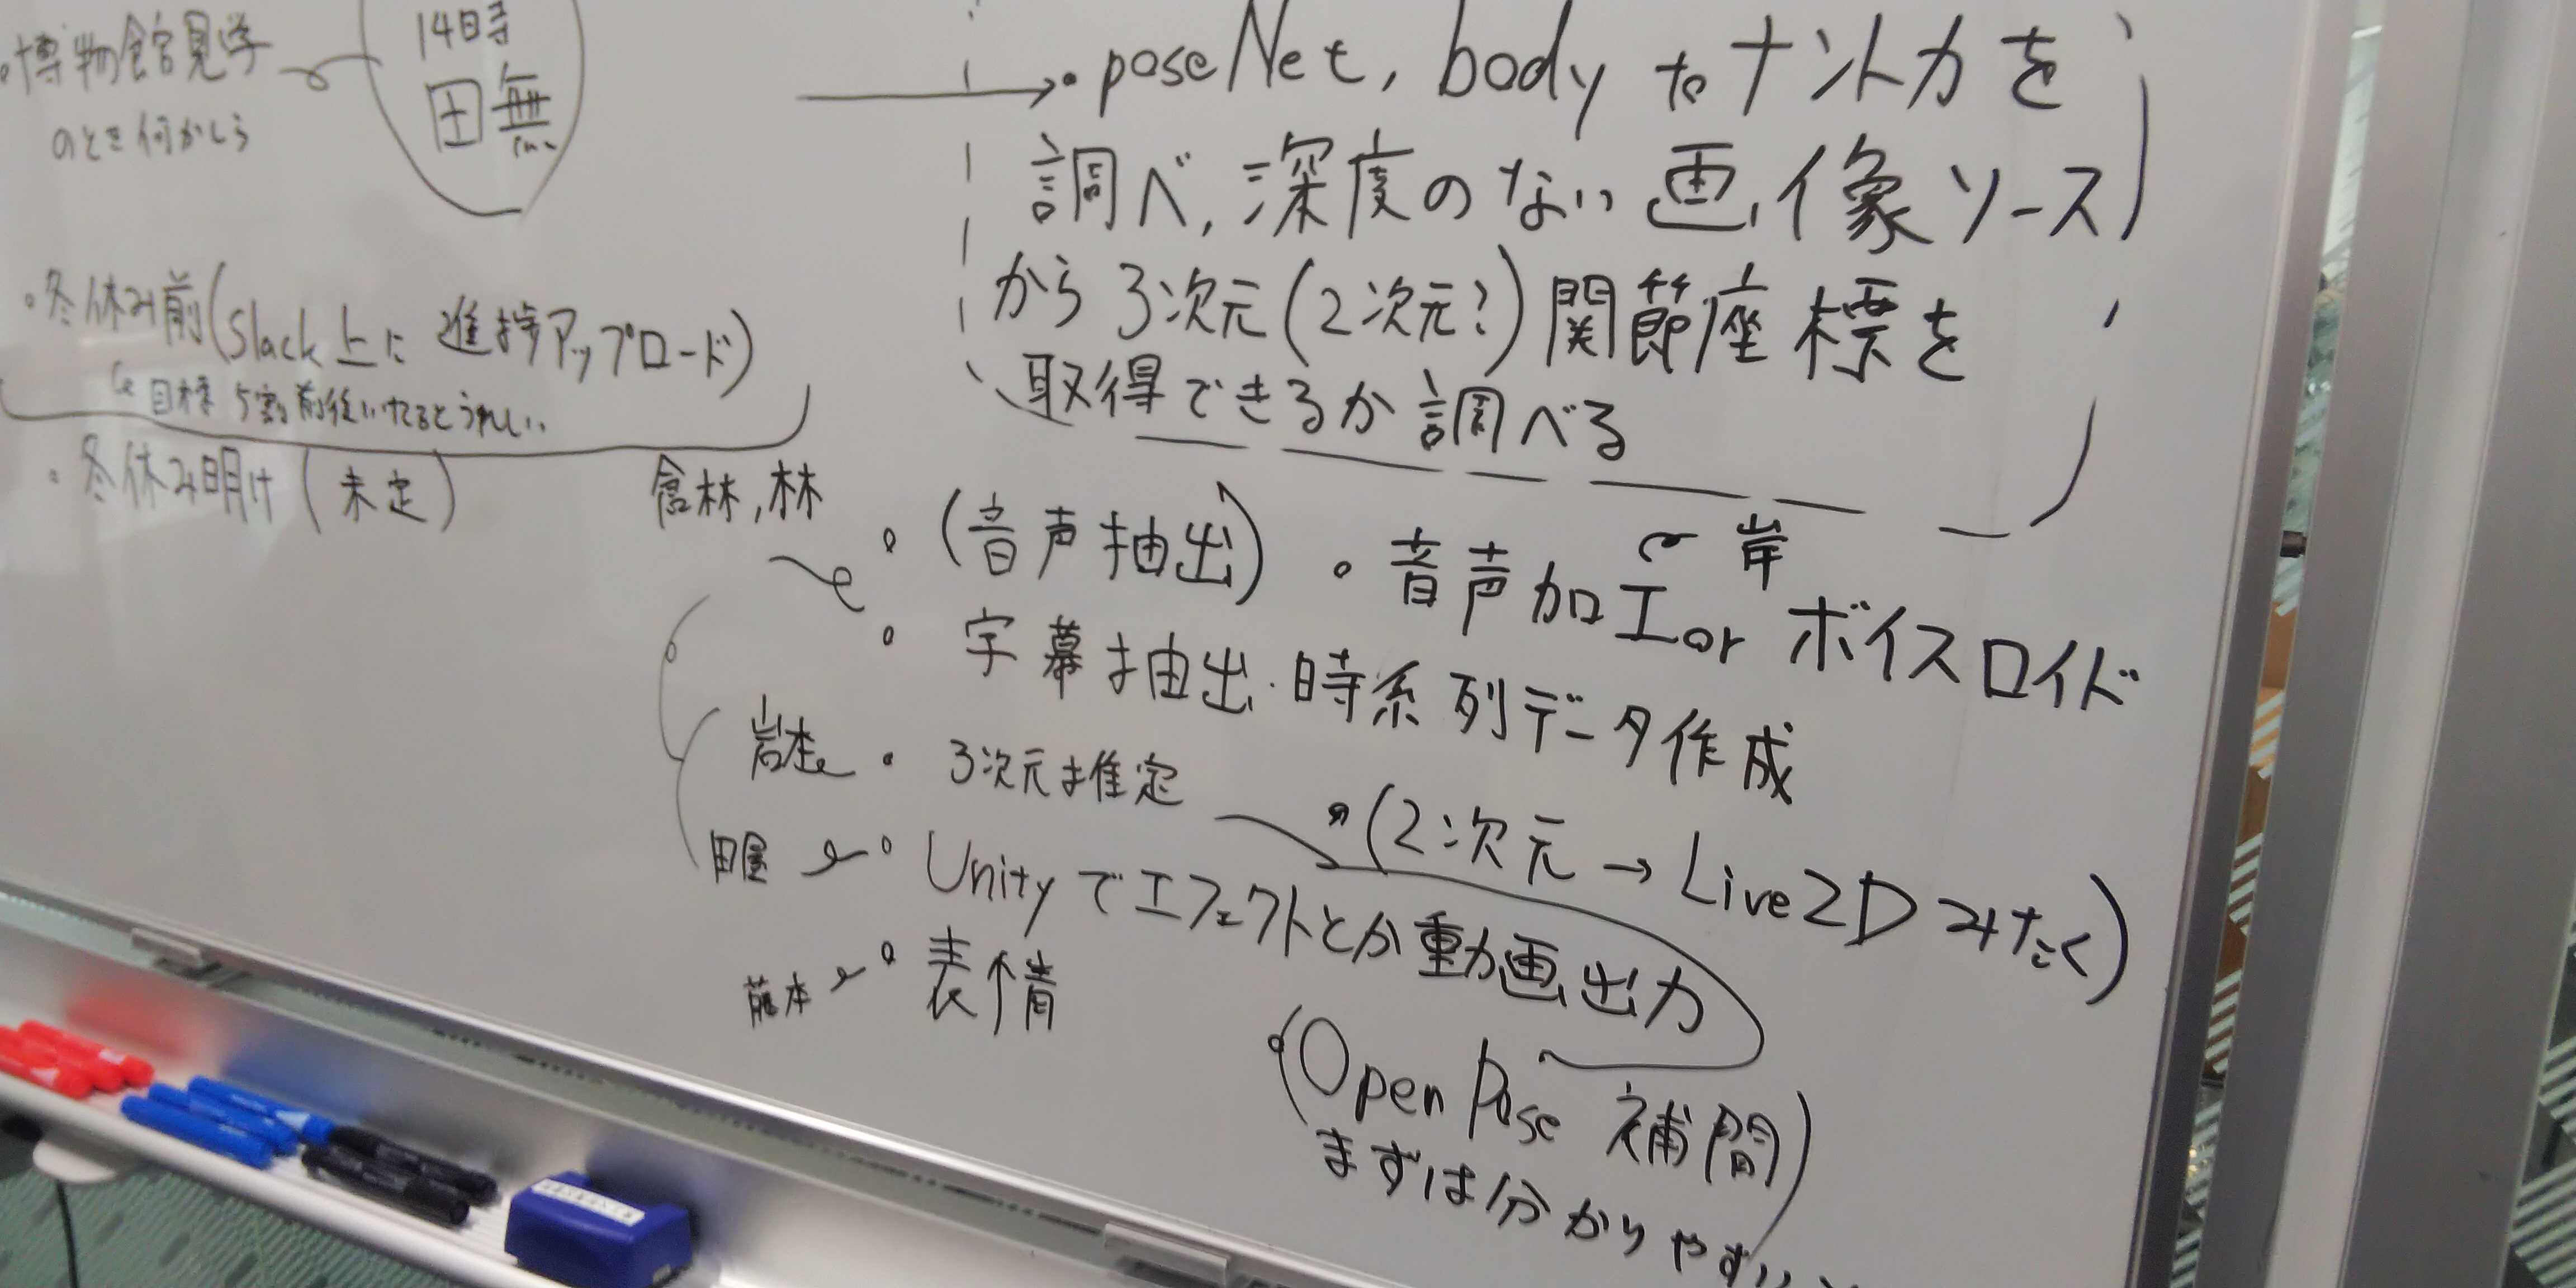
\includegraphics[width=1.0\textwidth]{fig/iw1322.png}
  \text{12月時点}
  \end{minipage}
 \caption{ミーティング内容の比較}
 \label{fig:iw132compare}
\end{figure}

\section{製作したハードウェア}
今プロジェクトでは、ハードウェアは作成していない。
\section{各種調査、分析レポート等}

\subsection{投票率低下の原因調査及びVtuber利用の妥当性の検討}

図\ref{fig:voterate}に示すように現代の日本では選挙率の低下が問題となっており、特に若者の投票率が低い。図\ref{fig:vote}に示された投票に行かなかった理由から、投票率の低下の原因の大きな一つとして政治への関心が低いことが考えられる。

\begin{figure}[H]
	\begin{center}
		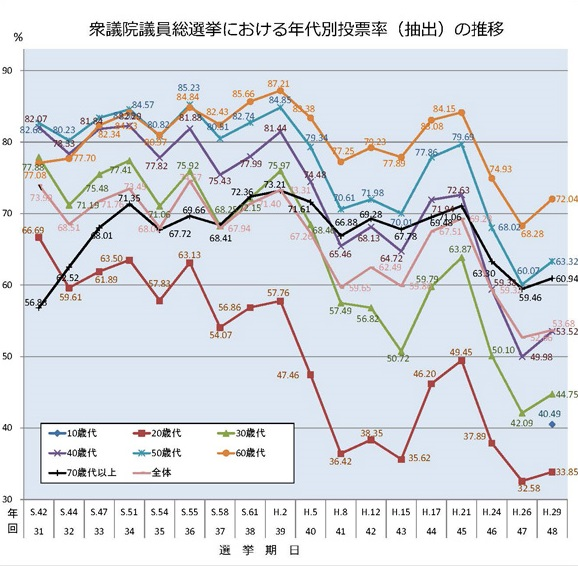
\includegraphics[width=12.0cm]{fig/voterate.jpg}
		\caption{投票率の推移(出典 総務省\cite{vote1})}
		\label{fig:voterate}
	\end{center}
\end{figure}

\begin{figure}[H]
	\begin{center}
		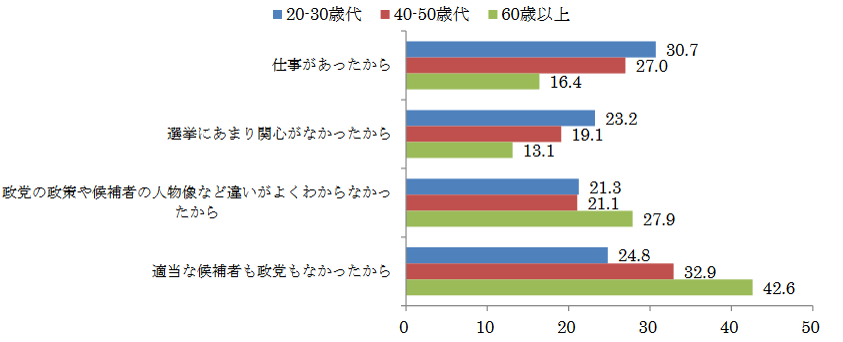
\includegraphics[width=12.0cm]{fig/vote.png}
		\caption{投票に行かなかった理由(出典 財団法人明るい選挙推進協会\cite{vote2})}
		\label{fig:vote}
	\end{center}
\end{figure}

若者の投票率を上げるためには、若者に認知度があり興味のあるVtuberと選挙を紐づけることが効果的であると考えた。図\ref{fig:vtuber}に示すようにVtuberは若者の間で圧倒的な認知度を得ている。このことからVtuberを利用することで、若者の選挙への関心度の増加が見込める。

\begin{figure}[H]
	\begin{center}
		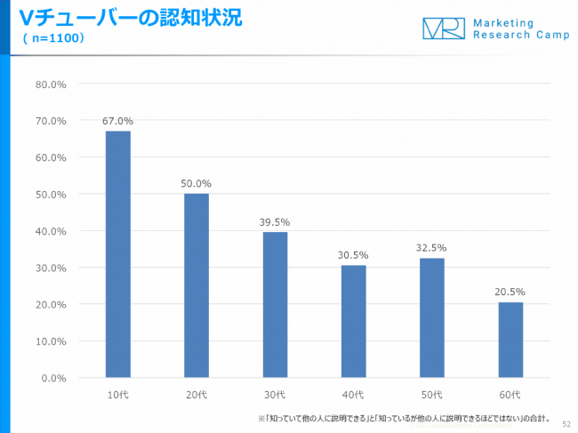
\includegraphics[width=12.0cm]{fig/vtube.png}
		\caption{VTuberの認知状況(出典 MoguLive\cite{vtuber})}
		\label{fig:vtuber}
	\end{center}
\end{figure}

\subsection{政見放送に関する権利等の調査}

本システムでは政見放送の動画編集を行うため、政見放送の著作権及び公職選挙法を考慮する必要がある。

政見放送は著作権法第40条の定める「公開して行なわれた政治上の演説又は陳述」にあたり、「いずれの方法によるかを問わず、利用することができる」と解される。つまり、二次的利用(27条)も許され、同一性保持権の侵害にならない限り翻訳や要約も許される。また、他に複製物を譲渡すること(26条の2)ができる\cite{law}。選挙期間中に政見放送がYouTube等の動画共有サイトにアップロードされることが問題になることがあるが、これは著作権法上ではなく公職選挙法上の問題である。例えば、特定の候補者の政見放送のみをアップロードすることにより公平性が担保できなくなる、などの理由が挙げられる\cite{wiki}。

つまり、内容の同一性が確保された範囲での編集は可能であり、公平性が担保されていれば政見放送を利用することは可能であると考えられる。

\subsection{Google Cloud Speech-to-Text の使用料金}

本システムで使用したGoogle colud Speech-to-Textは60分まで無料で使用できるが、超過すると課金が必要でありその内訳を表\ref{tab:GCS2T}に示す\cite{GCS2T}。ここで示す標準モデルは音声を対象としたモデルであり、プレミアムモデルは動画、拡張音声電話にも対象を拡張したモデルである。本システムでは一番安価なコースを用いた。約五分の政見放送を対象とすると一回の使用料金は約8円となる。なお、開発の際は無料期間を利用したため使用料金は発生しなかった。

\begin{table}[H]
	\begin{center}
		\begin{tabular}{c|c|c}
			機能&標準モデル&プレミアムモデル\\ \hline
			音声認識(データロギングなし)&\$0.006/15[s]&\$0.009/15[s]\\
			音声認識(データロギングあり)&\$0.004/15[s]&\$0.006/15[s]
		\end{tabular}
		\caption{Google Cloud Speech-to-Text使用料金}
		\label{tab:GCS2T}
	\end{center}
\end{table}

\section{発表資料}
\subsection{発表用スライド}
添付ファイルを参照のこと。

\subsection{課題設定発表での質疑応答一覧}

\begin{table}[H]
	\begin{tabular}{|l|l|} \hline
		{\bf 質問} & {\bf 回答} \\ \hline \hline
		骨格推定はできるか & Open Poseを用いることで可能 \\ \hline
		全員写すか, 1人にフォーカスするか & 1人にフォーカス\\ \hline
		各党でモデルを変えてはどうか & 公平性担保のためあまり変えない\\ \hline
		モデルは美少女のみか & はい\\ \hline
		可愛さのみで投票する恐れはないか & 各党でモデルに差異を付けない\\ \hline
		VTuber視聴割合のデータはあるか & 認知度のデータはある\\ \hline
		美少女でも討論は面白くないのでは & エフェクト等を工夫したい\\ \hline
		音声認識は難しいのでは & 字幕情報を使用する\\ \hline
		既存の政治解説VTuberとの差別化は & リアルタイムの用語解説を付加\\ \hline
		国会中継は動きがない & 動きのあるコンテンツを探す\\ \hline
		献血ポスターのように炎上する恐れ & 政治的中立性に則った上で関心を高めることが目的\\ \hline
	\end{tabular}
\end{table}

\subsection{中間発表での質疑応答一覧}

\begin{table}[H]
	\begin{tabular}{|l|l|} \hline
		{\bf 質問} & {\bf 回答} \\ \hline \hline
		国会中継から政見放送に変えたのか & 本システムを実装しやすいソースを選択した\\ \hline
		Open Poseの代替案(Pose Net等) & 検討する\\ \hline
		政見放送の権利問題, 著作権 & システムを政権に提供する形であれば問題なし\\ \hline
		他のものをソースにしてはどうか & エンタメ要素として活用できるため, 十分検討する\\ \hline
	\end{tabular}
\end{table}

\subsection{最終発表での質疑応答一覧}

\begin{table}[H]
	\begin{tabular}{|l|l|} \hline
		{\bf 質問} & {\bf 回答} \\ \hline \hline
		作成にあたり大変だった点はどこか & 開発言語が様々である各パートを組み合わせる点\\ \hline
	\end{tabular}
\end{table}

\begin{thebibliography}{99}
	\bibitem{vote1} 総務省|参議院議員通常選挙における年代別投票率の推移 \\\url{https://www.soumu.go.jp/senkyo/senkyo_s/news/sonota/nendaibetu/}
	\bibitem{vote2} 財団法人明るい選挙推進協会|第46回衆議院議員総選挙全国意識調査p39\\\url{http://www.akaruisenkyo.or.jp/wp/wp-content/uploads/2013/06/070seihon1.pdf}
	\bibitem{vtuber} MoguLive|VTuberを10代の約7割が認知 ジャストシステムがリサーチを発表	\\\url{https://www.moguravr.com/just-systems-vtuber-research/}
	\bibitem{law} 栗田隆:著作権法注釈\\\url{http://civilpro.law.kansai-u.ac.jp/kurita/copyright/commentary/Act40.html}
	\bibitem{wiki} Wikipedia|政見放送 \\\url{https://ja.wikipedia.org/wiki/政見放送}
	\bibitem{GCS2T} Google Cloud|Cloud Speech-to-Text ドキュメント-料金 \\\url{https://cloud.google.com/speech-to-text/pricing?hl=ja}

\end{thebibliography}

\end{document}
